%!TeX root=../monografia
%("dica" para o editor de texto: este arquivo é parte de um documento maior)
% para saber mais: https://tex.stackexchange.com/q/78101
\chapter{Rascunho Fusion Trees}
\label{cap:rascunho-fusion}

\section{Árvores B}

Uma árvore B, ou \textit{B-Tree}, é uma generalização da árvore binária de busca
perfeitamente balanceadas, em que um nó pode conter múltiplas chaves e ter mais
que dois filhos. É uma árvore auto balanceada e foi inventada por Rudolf Bayer e
Edward Meyers McCreight em 1971. 

Adotando a definição de Knuth, uma árvore B de ordem $b$ satisfaz as seguintes
propriedades:
\begin{itemize}
\item Cada nó tem no máximo $b$ filhos;
\item cada nó, com exceção da raiz e das folhas, tem pelo menos $\lceil
\frac{b}{2} \rceil$ filhos;
\item a raiz tem pelo menos 2 filhos, a não ser que seja uma folha;
\item todas as folhas tem o mesmo nível;
\item um nó com $k > 0$ filhos tem $k-1$ chaves.
\end{itemize}

A altura da árvore então é $\Theta(\log_b n)$. As operações de inserção/remoção
e predecessor/sucessor são feitas por meio de buscas na árvore, fazendo um pouco
de trabalho em cada nó. Vamos definir esse trabalho como $f(b)$ e, portanto, o
custo é 
\[
O(f(b) \log_b n).
\]

A busca funciona por meio da escolha de qual subárvore devemos descer. Ao buscar
por uma query $q$, quando chegamos em um nó, a subárvore que queremos é dada
pelo número de chaves naquele nó que são menores ou iguais que $q$. Definiremos
essa quantidade como o \textbf{rank}$(q)$. 

Podemos obter \textbf{rank}$(q)$ com uma busca linear, resultando em um custo de
$O(b \log_b n)$ para percorrer a árvore. Também podemos aplicar busca binária
nas chaves do nó, obtendo $O(\lg b \log_b n)=O(\lg n)$, uma complexidade
equivalente de uma ABBB.

Se conseguirmos determinar \textbf{rank}$(q)$ em tempo $O(1)$, teremos um custo
total das operações de apenas $O(\log_b n)$. 

\section{Visão inicial das Fusion Trees}

As Fusion Trees foram inventadas por Fredman e Willard em 1990 Elas utilizam de
diversas técnicas de manipulação de bits e paralelismo em nível de palavra para
obter uma complexidade de $O(\log_w n)$, onde $w$ é o número de bits em uma
\textit{palavra}, nas operações de busca. Vamos ver a fundo a versão estática
que conta com espaço linear em $n$ e precisa de um pré-processamento polinomial.
%~\cite{FrWi93}.

A ideia é construir uma árvore B com ordem $w^{1/5}$, lembrando que $w$ é o
tamanho da \textit{palavra}. Isso nos dá um nó com $k=O(w^{1/5})$ chaves
$x_0<x_1<\dots<x_{k-1}$. 

\textit{[...?]}

\section{Paralelismo em nível de palavra}

A técnica que vamos chamar de Paralelismo em nível de palavra
(\textit{Word-Level parallelism}) se aproveita do fato de estarmos no modelo
\textit{Word RAM}. Relembrando, nele as operações aritméticas e lógicas em
$\Theta(w)$ bits são executadas em tempo constante. Com um pouco de
criatividade, conseguimos aplicar funções que manipulam $\Omega(1)$ elementos
ainda em $O(1)$.

\subsection{Comparação paralela}

Podemos comparar duas \textit{bit strings} $x$ e $y$ de tamanho $s$ com uma
subtração. Para determinar se $x\geq y$, concatenamos um bit 1 ao início de $x$
e um 0 para $y$, depois fazemos a subtração dos valores. Por exemplo, para
$s=4$, $x=1100$ e $y=0011$, fazer a subtração de $1x$ e $0y$ nos dá:

\begin{figure}[h]
\bf \Large \centering
\begin{tabular}{cc}
& \textcolor{RawSienna}{1}\textcolor{Orange}{1100} \\
$-$ & \textcolor{blue}{0}\textcolor{cyan}{0011} \\
\hline
& \textcolor{Purple}{1}\textcolor{CarnationPink}{1001} 
\end{tabular}
\end{figure}

Se o valor do bit mais significativo no resultado é 1, então $x\geq y$. 

Conseguimos estender essa ideia para comparar múltiplas \textit{bit strings}
simultaneamente. Se temos dois arrays $A$ e $B$, cada um com 4 números de 4
bits:

\enlargethispage{2\baselineskip}

\begin{figure}[h]
\bf \Large \centering
\begin{tabular}{ccccc}
& $a_0$ & $a_1$ & $a_2$ & $a_3$ \\
\cline{2-5}
\textcolor{Orange}{$A$} = &
\multicolumn{1}{|c}{\textcolor{orange}{0100}} & \textcolor{orange}{1010} & \textcolor{orange}{0101} & \multicolumn{1}{c|}{\textcolor{orange}{0010}} \\
\cline{2-5} 
\hfill \\
& $b_0$ & $b_1$ & $b_2$ & $b_3$ \\
\cline{2-5}
\textcolor{cyan}{$B$} = &
\multicolumn{1}{|c}{\textcolor{cyan}{1111}} & \textcolor{cyan}{0111} & \textcolor{cyan}{0011} & \multicolumn{1}{c|}{\textcolor{cyan}{0001}} \\
\cline{2-5}
\end{tabular}
\end{figure}

Para fazer a comparação de todos os pares $a_i$ e $b_i$, adicionamos 1s entre os
valores de $A$ e 0s entre os de $B$. Por fim, fazemos a subtração e o bit que
precede $a_i-b_i$ é 1 se $a_i\geq b_i$ e 0 caso contrário:

\begin{figure}[h]
\bf \Large \centering
\begin{tabular}{cccccc}
& \textcolor{Orange}{$A$} &
\textcolor{RawSienna}{1}\textcolor{orange}{0100} & \textcolor{RawSienna}{1}\textcolor{orange}{1010} & \textcolor{RawSienna}{1}\textcolor{orange}{0101} & \textcolor{RawSienna}{1}\textcolor{orange}{0010} \\
$-$ & \textcolor{cyan}{$B$} &
\textcolor{blue}{0}\textcolor{cyan}{0010} &
\textcolor{blue}{0}\textcolor{cyan}{0100} &
\textcolor{blue}{0}\textcolor{cyan}{1000} &
\textcolor{blue}{0}\textcolor{cyan}{0001} \\
\hline
& \textcolor{CarnationPink}{$R$} &
\textcolor{Purple}{0}\textcolor{CarnationPink}{1011} & \textcolor{Purple}{1}\textcolor{CarnationPink}{0011} & \textcolor{Purple}{1}\textcolor{CarnationPink}{0010} & \textcolor{Purple}{1}\textcolor{CarnationPink}{0001} 
\end{tabular}
\end{figure}

Além disso, podemos aplicar uma máscara no resultado, restando apenas os bits
que nos interessam. Fazendo \textbf{AND} com uma \textit{palavra} com bits 1s
apenas nos bits que nos interessam da subtração, obtemos $R$:

\begin{figure}[h]
\bf \Large \centering
\begin{tabular}{c|cccc|}
\cline{2-5}
\textcolor{CarnationPink}{$R$} = &
\textcolor{Purple}{0}\textcolor{CarnationPink}{0000} & \textcolor{Purple}{1}\textcolor{CarnationPink}{0000} & \textcolor{Purple}{1}\textcolor{CarnationPink}{0000} & \textcolor{Purple}{1}\textcolor{CarnationPink}{0000} \\
\cline{2-5}
\end{tabular}
\end{figure}

Vamos definir então a operação \textbf{Comparação Paralela}$(A,B)$:

\textbf{Input:} Duas \textit{palavras} $A$ e $B$. $A$ contém um array de números
$a_0,\dots a_n$ com um bit de espaço entre cada número. O mesmo vale para $B$
com $b_0,\dots,b_n$.

\textbf{Output:} Uma \textit{palavra} $R$ com o resultado de $a_i\geq b_i$ nos
bits que ocupavam o espaço entre cada número nos arrays de input.



\textbf{Procedimento:}
\begin{itemize}
    \item Usar a operação \textbf{OR} para colocar 1 entre os valores de $A$.
    \item Usar a operação \textbf{AND} para colocar 0 entre os valores de $B$.
    \item Computar $A-B$ e aplicar uma máscara para obter apenas os bits que nos
    interessam com o resultado das comparações.
\end{itemize}

\subsection{Rank em $O(1)$}

Lembre-se, que nosso objetivo é: dada uma consulta $q$, saber em tempo constante
qual a subárvore que devemos descer dentre as possíveis de um nó da Fusion Tree.
Para isso, queremos determinar o rank de $q$ em relação à todas as chaves de um
nó, isso na prática significa fazer a comparação entre $q$ e cada uma das
chaves. 

Se conseguirmos colocar as chaves do nó em um array e $q$ repetidas vezes em
outro, ambos adequados para a \textbf{Comparação Paralela}, então conseguimos
fazer toda a comparação de uma vez só. Contando o número de 1s nos bits
``sentinela'' \textit{[nome melhor para dar?]} , conseguimos determinar quantas
chaves são $\leq q$, ou seja, seu rank.

\subsection{Parallel Tile}

\textit{[Ladrilhamento paralelo? Blocagem? ]}

Para obter uma palavra com múltiplas cópias de uma mesma \textit{bit string} $q$
interespaçadas por um bit, precisamos fazer uma multiplicação com um número
específico que distribua $q$ igualmente. Por exemplo, para $q=1100$ e um tamanho
de palavra de 20 bits, queremos obter:

\begin{figure}[h]
\bf \Large \centering
\begin{tabular}{|cccc|}
\hline
\textcolor{RawSienna}{0}\textcolor{Orange}{1100} &
\textcolor{RawSienna}{0}\textcolor{Orange}{1100} &
\textcolor{RawSienna}{0}\textcolor{Orange}{1100} & \textcolor{RawSienna}{0}\textcolor{Orange}{1100} \\
\hline
\end{tabular}
\end{figure}

A resposta nesse caso é usar $M=00001000010000100001$. A operação $q\times M=R$
nos dá:

\begin{figure}[h]
\bf \Large \centering
\begin{tabular}{cccccc}
& \textcolor{Orange}{$q$} & & & &
\textcolor{Orange}{\phantom{0}1100} \\
$\times$ & \textcolor{Red}{M} &
\textcolor{RawSienna}{0}\textcolor{Red}{0001} &
\textcolor{RawSienna}{0}\textcolor{Red}{0001} &
\textcolor{RawSienna}{0}\textcolor{Red}{0001} & \textcolor{RawSienna}{0}\textcolor{Red}{0001} \\
\hline
& & & & & 
\textcolor{RawSienna}{0}\textcolor{Orange}{1100} \\
& & & & 
\textcolor{RawSienna}{0}\textcolor{Orange}{1100} &
\textcolor{gray}{00000} \\
& & & 
\textcolor{RawSienna}{0}\textcolor{Orange}{1100} &
\textcolor{gray}{00000} &
\textcolor{gray}{00000} \\
$+$ & & 
\textcolor{RawSienna}{0}\textcolor{Orange}{1100} & 
\textcolor{gray}{00000} & 
\textcolor{gray}{00000} & 
\textcolor{gray}{00000} \\
\hline
& \textcolor{RawSienna}{R} &
\textcolor{RawSienna}{0}\textcolor{Orange}{1100} &
\textcolor{RawSienna}{0}\textcolor{Orange}{1100} &
\textcolor{RawSienna}{0}\textcolor{Orange}{1100} & \textcolor{RawSienna}{0}\textcolor{Orange}{1100} \\
\end{tabular}
\end{figure}

Note que, em $M$, colocamos bits $1$ apenas nos bits mais a direita de onde
queremos que inicie cada cópia de $q$. Isso fez com que cada linha seja um shift
a esquerda $q$. O tamanho do shift é determinado pelo índice daquele bit 1.
Então, colocando esses bits em intervalos de $\len(q)+1$, ao fazer a soma das
linhas, obtemos várias cópias em sequência, espaçadas pelos bits sentinela.

\textit{[não sei se gostei dessa explicação]}

Além disso, podemos fazer com que os bits sentinela tenham valor 1 de forma
simples. Um \textbf{OR} com uma palavra que contenha bits 1 apenas nos mesmos
índices que os sentinela sobtém isso. No nosso exemplo, seria $Q = R$
\textbf{OR} $1000100010001000$. Obtendo afinal:


\begin{figure}[h]
\bf \Large \centering
\begin{tabular}{c|cccc|}
\cline{2-5}
\textcolor{Orange}{$Q$} = &
\textcolor{RawSienna}{1}\textcolor{Orange}{1100} &
\textcolor{RawSienna}{1}\textcolor{Orange}{1100} &
\textcolor{RawSienna}{1}\textcolor{Orange}{1100} & \textcolor{RawSienna}{1}\textcolor{Orange}{1100} \\
\cline{2-5}
\end{tabular}
\end{figure}

Definimos a operação \textbf{Parallel Tile}$(q)$:

\textbf{Input:} Número $q$ menor que uma palavra

\textbf{Output:} Uma palavra contendo múltiplas cópias de $q$ interespaçadas por
um bit 1.

\textbf{Procedimento:} 
\begin{itemize}
    \item Formar um número $M$ com um bit $1$ no bit mais à direita de cada
    cópia desejada de $q$. 
    \item Fazer a multiplicação $q\times M = R$
    \item Retornar $Q$, o resultado de $R$ \textbf{OR} uma palavra que contenha
    bits 1 no índice dos bits sentinelas de $R$. 
\end{itemize} 

\textit{[Obs: o resultado vai formar uma palavra perfeitamente, mesmo se $\len(q)+1$ não é múltiplo de $w$?]}

\subsection{Soma Paralela}

\hfill

Dado o resultado $Q$ do \textbf{Parallel Tile} de uma consulta $q$ e as chaves
do nó reunidas em um array adequado $X$, intercalados por bits 0, podemos
realizar a operação de \textbf{Comparação Paralela}. O resultado fica armazenado
em uma palavra que nomeamos $R$:

\begin{figure}[h]
\bf \Large \centering
\begin{tabular}{cccccc}
\large{Comparação} & \textcolor{Orange}{$Q$} &
\textcolor{RawSienna}{1}\textcolor{orange}{1100} &
\textcolor{RawSienna}{1}\textcolor{orange}{1100} &
\textcolor{RawSienna}{1}\textcolor{orange}{1100} &
\textcolor{RawSienna}{1}\textcolor{orange}{1100} \\
\large{Paralela} & \textcolor{cyan}{$X$} &
\textcolor{blue}{0}\textcolor{cyan}{0001} &
\textcolor{blue}{0}\textcolor{cyan}{0101} &
\textcolor{blue}{0}\textcolor{cyan}{1011} &
\textcolor{blue}{0}\textcolor{cyan}{1101} \\
\hline
& \textcolor{CarnationPink}{$R$} & 
\textcolor{Purple}{1}\textcolor{CarnationPink}{0000} & \textcolor{Purple}{1}\textcolor{CarnationPink}{0000} & \textcolor{Purple}{0}\textcolor{CarnationPink}{0000} & \textcolor{Purple}{0}\textcolor{CarnationPink}{0000} 
\end{tabular}
\end{figure}

Queremos de alguma forma somar o número de bits sentinela iguais a 1. Essa
quantidade, é o \textbf{rank}$(q)$. Generalizando, nós temos bits de interesse
$a,b,c,d$ igualmente espaçados numa palavra com todos os outros bits iguais a 0,
como na Figura~\ref{f:bits-de-interesse}.

\begin{figure}[h]
\bf \Large \centering
\begin{tabular}{cccc}
\textcolor{Purple}{a}\textcolor{CarnationPink}{0000} &
\textcolor{Purple}{b}\textcolor{CarnationPink}{0000} &
\textcolor{Purple}{c}\textcolor{CarnationPink}{0000} &
\textcolor{Purple}{d}\textcolor{CarnationPink}{0000}
\end{tabular}
\label{f:bits-de-interesse}
\end{figure}

Uma ideia simples, seria percorrer por toda a palavra e ir somando os bits.
Contudo, isso tomaria tempo proporcional ao tamanho da palavra. Nós queremos
fazer em tempo $O(1)$. Para isso, vamos utilizar um multiplicador adequado que
vai computar $a+b+c+d$ para nós. Se, de forma similar ao \textbf{Parallel Tile},
a multiplicação nos dar shifts adequados, conseguimos concentrar a soma dos bits
de interesse em um só lugar:

\begin{figure}[h]
\bf \Large \centering
\begin{tabular}{cccccccc}
& & & & \textcolor{Purple}{a}\textcolor{CarnationPink}{0000} &
\textcolor{Purple}{b}\textcolor{CarnationPink}{0000} &
\textcolor{Purple}{c}\textcolor{CarnationPink}{0000} &
\textcolor{Purple}{d}\textcolor{CarnationPink}{0000} \\
& & & \textcolor{Purple}{a}\textcolor{CarnationPink}{0000} &
\textcolor{Purple}{b}\textcolor{CarnationPink}{0000} &
\textcolor{Purple}{c}\textcolor{CarnationPink}{0000} &
\textcolor{Purple}{d}\textcolor{CarnationPink}{0000} &
\textcolor{gray}{00000} \\
& & \textcolor{Purple}{a}\textcolor{CarnationPink}{0000} &
\textcolor{Purple}{b}\textcolor{CarnationPink}{0000} &
\textcolor{Purple}{c}\textcolor{CarnationPink}{0000} &
\textcolor{Purple}{d}\textcolor{CarnationPink}{0000} &
\textcolor{gray}{00000} &
\textcolor{gray}{00000} \\
$+$ & \textcolor{Purple}{a}\textcolor{CarnationPink}{0000} & \textcolor{Purple}{b}\textcolor{CarnationPink}{0000} &
\textcolor{Purple}{c}\textcolor{CarnationPink}{0000} & 
\textcolor{Purple}{d}\textcolor{CarnationPink}{0000} & 
\textcolor{gray}{00000} & 
\textcolor{gray}{00000} & 
\textcolor{gray}{00000} \\
\hline
& \textcolor{lightgray}{?????} &
\textcolor{lightgray}{?????} & 
\textcolor{lightgray}{????}\textcolor{Green}{s} & 
\textcolor{Green}{s}\textcolor{lightgray}{????} & 
\textcolor{lightgray}{?????} &
\textcolor{lightgray}{?????} & 
\textcolor{lightgray}{?????}
\end{tabular}
\end{figure}

Aqui, os dois bits indicados por \textbf{\textcolor{Green}{ss}} contém o valor
da soma \textbf{\textcolor{Purple}{a}} $+$ \textbf{\textcolor{Purple}{b}} $+$
\textbf{\textcolor{Purple}{c}} $+$ \textbf{\textcolor{Purple}{d}}.

Note que o multiplicador deve novamente espaçar os shifts no tamanho de $q+1$,
como foi feito no \textbf{Parallel Tile}. A diferença é que lá esse shift era
aplicado a uma \textit{bit-string} de tamanho $q$ e por isso ela era copiada
repetidas vezes sem somar nada. Aqui, temos \textit{bit-strings} de tamanho
$\len(q)+1$, pois o bit sentinela já está incluso, assim o shift força a soma
dos sentinela. No nosso exemplo, com uma palavra de tamanho 20, o multiplicador
precisa ser $M=00001000010000100001$.

Essa multiplicação dará a soma que nos interessa na posição dos bits mais
significativos da palavra original. Fazendo um shift para a direita e uma
máscara de 1s (a máscara deve ser de tamanho igual ao número de bits que nos
interessam), obtemos por fim um valor que nos dá o \textbf{rank}(q).

\textbf{Soma Paralela}$(R)$

\textbf{Input:} Uma \textit{palavra} $R$ com bits de interesse equiespaçados,
separados por bits 0.

\textbf{Output:} A soma dos bits de interesse.

\textbf{Procedimento:} 
\begin{itemize}
\item Realizar um \textbf{Parallel Tile} com um multiplicador apropriado para
empilhar todos os bits de interesse em uma mesma soma. 
\item Usar um shift e uma máscara para obter o resultado final.
\end{itemize}

\subsection{Rank Paralelo}

Com essas operações, conseguimos computar o rank de uma \textit{query} $q$ entre
as chaves de um nó em tempo constante. Estamos supondo que $\len(q) = \len(x_i)$
onde $x_i$ é uma chave do nó. Além disso, para que tudo funcione, o tamanho
dessas \textit{bit-strings} precisa ser muito menor que o tamanho da palavra
$w$, de forma que todas as chaves $x_i$ de um nó cabem intercaladas por um bit
em um array de tamanho $w$, para podermos realizar a \textbf{Comparação
Paralela}.

\textbf{Rank Paralelo}$(q)$

\textbf{Input:} Um array de inteiros $X = x_1,\dots x_n$ numa \textit{palavra}
com um bit de espaço entre eles. Uma query $q$.

\textbf{Output:} O número de elementos no array que é menor ou igual a $q$.

\textbf{Procedimento:}
\begin{itemize}
    \item Realizar um \textbf{Parallel Tile} na \textit{query} $q$ para obter um
    array com $n$ cópias de $q$ espaçadas por bits 1.
    \item Realizar uma \textbf{Comparação Paralela} entre o array de $q$ e $X$.
    \item Realizar uma \textbf{Soma Paralela} para obter o \textbf{rank}$(q)$.
\end{itemize}

\subsection{Bit Mais Significativo}

O problema do \textit{Most Significant Set Bit}, ou MSB, é um clássico na
computação. A operação $MSB(X)$ retorna o índice do bit 1 mais a direita de $x$.
Em muitas arquiteturas, uma única instrução de Assembly calcula esse valor. Em
x86, a instrução se chama BSR (\textit{Bit Scan Reverse}).

Contudo, no nosso modelo de máquina, podemos usar apenas os operadores simples
do C. Dessa forma, vamos partir das técnicas vistas até agora para construir um
algoritmo que computa o MSB em uma \textit{palavra} de tamanho $w$ em $O(1)$.

Primeiro, podemos notar que se MSB$(w) = k$, então $2^k\geq n$. Assim,
determinar o rank de $w$ entre todas as potências de 2 até $2^w$ nos dá o
MSB$(w)$. O problema é que um array com todas essas potências de $2$ não cabe em
uma palavra, isso na verdade ocuparia $\Theta(w^2)$ bits.

Para resolver isso, a ideia central é que precisamos dividir nossa palavra $w$
em blocos menores, que consigamos comparar com potências de $2$ que ainda cabem
em uma palavra. Dividindo $w$ em clusters, se conseguirmos encontrar o primeiro
cluster não vazio, precisamos achar o primeiro bit 1 apenas dentro desse
cluster.

Se vamos dividir $w$ em clusters de tamanho $b$, a questão é que valor de $b$
minimiza o $\max \{b,\frac{w}{b}\}$? A resposta é $b=w^{1/2}$. Para identificar
clusters não-vazios, vamos construir um bit-string com tamanho igual ao número
de clusters, em que cada bit indica se aquele cluster está vazio ou não. Teremos
uma estrutura como:

\textit{[Como chegamos que $1/2$ minimiza a equação? - Falar isso na seção da vEB]}

\begin{figure}[h]
\centering
\begin{tikzpicture}

    % 1. Array Base A
    \def\w{16}
    \def\bitvals{0,0,0,0,0,0,1,0,1,0,1,0,0,0,0,0}
    \foreach \val [count=\i from 0] in \bitvals {
        \ifthenelse{\i>3 \and \i<8}{
            \ifthenelse{\i=6}{
                \node[array cell, fill=orange] (A) at ($(0,0) + (\i*0.55, 0)$) {\val};
            }{
                \node[array cell, fill=yellow] (A) at ($(0,0) + (\i*0.55, 0)$) {\val};
            }
        }{
            \node[array cell] (A\i) at ($(0,0) + (\i*0.55, 0)$) {{\val}};
        }
        \pgfmathtruncatemacro{\idx}{\w - 1 - \i}
        \node[array index, below=of A\i] {\idx};
    }
    \node[left=0.2cm of A0] {$A$};

    % 2. Linhas verticais grossas de divisão de Clusters (a cada 4 elementos)
    \foreach \x in {3, 7, 11} {
        \draw[cluster split] ($(A\x.north east)+(0, 0.1)$) -- ($(A\x.south east)-(0, 0.1)$);
    }

    % 3. Braces (chaves) sobre os clusters
    \draw[cluster brace] (A0.north west) -- (A3.north east) 
        node[midway, above=4pt] (b0) {};
    \draw[cluster brace] (A4.north west) -- (A7.north east) 
        node[midway, above=4pt] (b1) {};
    \draw[cluster brace] (A8.north west) -- (A11.north east) 
        node[midway, above=4pt] (b2) {};
    \draw[cluster brace] (A12.north west) -- (A15.north east) 
        node[midway, above=4pt] (b3) {};

    % Rotulo \sqrt{w} bits
    \node[above right=2pt and -10pt of b3, font=\small] {$\sqrt{w}\text{ bits}$};

    % 4. Array de Summary
    % Posicionado acima do ponto médio do vetor A
    \path ($(A0.north)!.5!(A15.north)$) ++(-0.825, 2.0) coordinate (sum_pos);

    \def\sqrtw{4}
    \foreach \val [count=\i from 0] in {0, 1, 0, 1} {
        \ifnum\i=1
            \node[array cell, fill=yellow] (sum\i) at ($(sum_pos) + (\i*0.55, 0)$) {\val};
        \else
            \node[array cell] (sum\i) at ($(sum_pos) + (\i*0.55, 0)$) {\val};
        \fi
        \pgfmathtruncatemacro{\idx}{\sqrtw - 1 - \i}
        \node[array index, above=of sum\i] {\idx};
    }
    \node[left=0.2cm of sum0, font=\itshape] {summary};
    \node[right=0.2cm of sum3, font=\small] {$\sqrt{w}\text{ bits}$};

    % 5. Conexões entre o Summary e os Braces
    \draw (sum0.south) -- (b0.north);
    \draw (sum1.south) -- (b1.north);
    \draw (sum2.south) -- (b2.north);
    \draw (sum3.south) -- (b3.north);

\end{tikzpicture}
\end{figure}
\textit{[Figura copiada da parte da vEB, pensar se vale tentar construir uma estrutura diferente depois]}

Como cada cluster tem tamanho $\sqrt w$, para determinar seu bit mais
significativo, precisamos fazer um \textbf{rank} dos bits daquele cluster em
relação a um array de $\sqrt w$ potências de 2. Cada uma dessas potências de 2
ocupa $\sqrt{w}$ bits, mas para construir nosso array de \textbf{Comparação
Paralela}, o bit que interespaça as potências vai acabar tornando o array final
de tamanho maior que $w$. 

Nesse ponto, a questão se torna como podemos contornar esse problema. Uma
possibilidade é dividir as potências de 2 em dois arrays diferentes e computar o
\textbf{rank} duas vezes. Outra, é tratar o bit mais significativo como um caso
especial, sobrando apenas $\sqrt{w}-1$ bits para comparar. De qualquer forma, o
tempo constante para a operação se mantém.

\subsubsection{Identificando clusters não-vazios}

Como exemplo, vamos supor que temos uma palavra $X=0101000010001101$ de tamanho
$w=16$. Seus clusters então são da forma:

\begin{figure}[h]
 \bf \Large\centering
 \begin{tabular}{c|cccc|}
\cline{2-5}
\textcolor{PineGreen}{$X$} = &
\textcolor{PineGreen}{0101} &
\textcolor{PineGreen}{0000} &
\textcolor{PineGreen}{1000} &
\textcolor{PineGreen}{1101} \\
\cline{2-5}
  \end{tabular}
\end{figure}

A ideia que vamos aplicar para identificar se um clusters está vazio ou não é
inicialmente verificar se o seu primeiro bit é 1. Depois, checar se algum dos
bits restantes, no caso os 3 últimos, contém um 1. Para começar então, aplicamos
uma máscara que contém bit 1 apenas no primeiro bit de cada cluster, denominamos
ela como $F$:

\begin{figure}[h]
 \bf \Large\centering
 \begin{tabular}{c|cccc|}
\cline{2-5}
\textcolor{orange}{$F$} = &
\textcolor{orange}{1000} &
\textcolor{orange}{1000} &
\textcolor{orange}{1000} &
\textcolor{orange}{1000} \\
\cline{2-5}
  \end{tabular}
\end{figure}

Fazemos então $X$ \textbf{AND} $F$ obtendo $R$:

\begin{figure}[h]
 \bf \Large\centering
 \begin{tabular}{cccccc}
& \textcolor{PineGreen}{$X$} &
\textcolor{PineGreen}{0101} &
\textcolor{PineGreen}{0000} &
\textcolor{PineGreen}{1000} &
\textcolor{PineGreen}{1101} \\
AND & \textcolor{orange}{$F$} &
\textcolor{orange}{1000} &
\textcolor{orange}{1000} &
\textcolor{orange}{1000} &
\textcolor{orange}{1000} \\
      \hline
& \textcolor{Violet}{$R_1$} &
\textcolor{Violet}{0}\textcolor{DarkOrchid}{000} &
\textcolor{Violet}{0}\textcolor{DarkOrchid}{000} &
\textcolor{Violet}{1}\textcolor{DarkOrchid}{000} &
\textcolor{Violet}{1}\textcolor{DarkOrchid}{000}
 \end{tabular}
\end{figure}

Com $R_1$, indicamos pelo primeiro bit de cada cluster se o primeiro bit está
setado. Agora fazemos $X$ \textbf{XOR} $R_1$ obtendo $R_2$: 

\begin{figure}[h]
 \bf \Large\centering
 \begin{tabular}{cccccc}
& \textcolor{PineGreen}{$X$} &
\textcolor{PineGreen}{0101} &
\textcolor{PineGreen}{0000} &
\textcolor{PineGreen}{1000} &
\textcolor{PineGreen}{1101} \\
XOR & \textcolor{Violet}{$R_1$} &
\textcolor{Violet}{0}\textcolor{DarkOrchid}{000} &
\textcolor{Violet}{0}\textcolor{DarkOrchid}{000} &
\textcolor{Violet}{1}\textcolor{DarkOrchid}{000} &
\textcolor{Violet}{1}\textcolor{DarkOrchid}{000} \\
      \hline
& \textcolor{blue}{$R_2$} &
\textcolor{blue}{0}\textcolor{PineGreen}{101} &
\textcolor{blue}{0}\textcolor{PineGreen}{000} &
\textcolor{blue}{0}\textcolor{PineGreen}{000} &
\textcolor{blue}{0}\textcolor{PineGreen}{101} 
 \end{tabular}
\end{figure}

Note que $R_2$ contém os últimos 3 bits de cada cluster original de $X$, mas
separados por um bit 0. Podemos fazer a \textbf{Comparação Paralela} com $F$,
que nessa perspectiva é composto por várias bitstrings com valor zero
intercaladas com 1 para a comparação. O que vamos obter como resultado dessa
comparação, é saber se cada um dos clusters de $R_2$ tem valor maior que 0, ou
seja, se tem pelo menos um bit 1. Isso será indicado pelos bits sentinela,
aqueles com valor 0 são dos clusters não vazios. Queremos indicar com um bit 1
os clusters não vazios, então simplesmente fazemos um \textbf{XOR} com $F$,
obtendo afinal $R_3$:

\begin{figure}[h]
\bf \Large \centering
\begin{tabular}{cccccc}
\large{Comparação} & \textcolor{orange}{$F$} &
\textcolor{RawSienna}{1}\textcolor{orange}{000} &
\textcolor{RawSienna}{1}\textcolor{orange}{000} &
\textcolor{RawSienna}{1}\textcolor{orange}{000} &
\textcolor{RawSienna}{1}\textcolor{orange}{000} \\
\large{Paralela} & \textcolor{blue}{$R_2$} &
\textcolor{blue}{0}\textcolor{PineGreen}{101} &
\textcolor{blue}{0}\textcolor{PineGreen}{000} &
\textcolor{blue}{0}\textcolor{PineGreen}{000} &
\textcolor{blue}{0}\textcolor{PineGreen}{101} \\
\hline
& &
\textcolor{Purple}{0}\textcolor{CarnationPink}{000} &
\textcolor{Purple}{1}\textcolor{CarnationPink}{000} &
\textcolor{Purple}{1}\textcolor{CarnationPink}{000} &
\textcolor{Purple}{0}\textcolor{CarnationPink}{000} \\
\large{XOR} & \textcolor{orange}{$F$} &
\textcolor{RawSienna}{1}\textcolor{orange}{000} &
\textcolor{RawSienna}{1}\textcolor{orange}{000} &
\textcolor{RawSienna}{1}\textcolor{orange}{000} &
\textcolor{RawSienna}{1}\textcolor{orange}{000} \\
\hline
& \textcolor{Purple}{$R_3$} &
\textcolor{Purple}{1}\textcolor{CarnationPink}{000} &
\textcolor{Purple}{0}\textcolor{CarnationPink}{000} &
\textcolor{Purple}{0}\textcolor{CarnationPink}{000} &
\textcolor{Purple}{1}\textcolor{CarnationPink}{000} \\
\end{tabular}
\end{figure}

Agora, o primeiro bit de cada cluster em $R_1$ nos diz se o primeiro bit daquele
cluster em $X$ está setado. Já os de $R_3$ nos dizem se pelo menos um dos bits
restantes naquele cluster está. Com um simples \textbf{OR}, conseguimos uma
bitstring $R$ que informa se cada cluster de $X$ tem um bit 1 ou não:

\begin{figure}[h]
\bf \Large \centering
\begin{tabular}{cccccc}
& \textcolor{Purple}{$R_3$} &
\textcolor{Purple}{1}\textcolor{CarnationPink}{000} &
\textcolor{Purple}{0}\textcolor{CarnationPink}{000} &
\textcolor{Purple}{0}\textcolor{CarnationPink}{000} &
\textcolor{Purple}{1}\textcolor{CarnationPink}{000} \\
\large{OR} & \textcolor{Violet}{$R_1$} &
\textcolor{Violet}{0}\textcolor{DarkOrchid}{000} &
\textcolor{Violet}{0}\textcolor{DarkOrchid}{000} &
\textcolor{Violet}{1}\textcolor{DarkOrchid}{000} &
\textcolor{Violet}{1}\textcolor{DarkOrchid}{000} \\
\hline
& \textcolor{PineGreen}{$C$} & 
\textcolor{PineGreen}{1}\textcolor{LimeGreen}{000} &
\textcolor{PineGreen}{0}\textcolor{LimeGreen}{000} &
\textcolor{PineGreen}{1}\textcolor{LimeGreen}{000} &
\textcolor{PineGreen}{1}\textcolor{LimeGreen}{000} 
\end{tabular}
\end{figure}

Queremos, contudo, obter uma bit-string com apenas os bits de interesse. Para
isso, vamos relembrar de como construímos a técnica da \textbf{Soma Paralela},
fazendo uma multiplicação que gera shifts especificamente para empilhar os bits
de interesse e somá-los ao final. A diferença é que agora nosso objetivo é
concatenar esses bits, buscamos que nossa multiplicação faça algo da forma:

\begin{figure}[h]
\bf \Large \centering
\begin{tabular}{cccccccc}
& & & & \textcolor{PineGreen}{1}\textcolor{LimeGreen}{000} &
\textcolor{PineGreen}{0}\textcolor{LimeGreen}{000} &
\textcolor{PineGreen}{1}\textcolor{LimeGreen}{000} &
\textcolor{PineGreen}{1}\textcolor{LimeGreen}{000} \\
& & & \textcolor{PineGreen}{\phantom{0}1}\textcolor{LimeGreen}{00} & 
\textcolor{LimeGreen}{0}\textcolor{PineGreen}{0}\textcolor{LimeGreen}{00} &
\textcolor{LimeGreen}{0}\textcolor{PineGreen}{1}\textcolor{LimeGreen}{00} &
\textcolor{LimeGreen}{0}\textcolor{PineGreen}{1}\textcolor{LimeGreen}{00} &
\textcolor{LimeGreen}{0}\textcolor{gray}{000} \\
& & \textcolor{PineGreen}{\phantom{00}1}\textcolor{LimeGreen}{0} &
\textcolor{LimeGreen}{00}\textcolor{PineGreen}{0}\textcolor{LimeGreen}{0}  &
\textcolor{LimeGreen}{00}\textcolor{PineGreen}{1}\textcolor{LimeGreen}{0}  &
\textcolor{LimeGreen}{00}\textcolor{PineGreen}{1}\textcolor{LimeGreen}{0}  &
\textcolor{LimeGreen}{00}\textcolor{gray}{00} &
\textcolor{gray}{0000} \\
$+$ & \textcolor{PineGreen}{\phantom{000}1} &
\textcolor{LimeGreen}{000}\textcolor{PineGreen}{0} &
\textcolor{LimeGreen}{000}\textcolor{PineGreen}{1} &
\textcolor{LimeGreen}{000}\textcolor{PineGreen}{1} &
\textcolor{LimeGreen}{000}\textcolor{gray}{0} &
\textcolor{gray}{0000} &
\textcolor{gray}{0000} \\
\hline
& \textcolor{lightgray}{????} &
\textcolor{lightgray}{????} & 
\textcolor{lightgray}{????} & 
\textcolor{PineGreen}{1011} & 
\textcolor{lightgray}{????} &
\textcolor{lightgray}{????} & 
\textcolor{lightgray}{????}
\end{tabular}
\end{figure}

A técnica para fazer isso se chama \textbf{Sketching} e será vista mais a fundo
na próxima seção. Por ora, podemos ter a intuição que precisamos realizar shifts
de tamanho igual ao número de bits que não nos interessam. Nesse caso, são 3
bits, então simplesmente precisamos de uma \textit{bit-string} que tenha um bit
1 nas posições $0,3$ e 6, $M=001001001$.

Os bits que nos interessam estarão posicionados no cluster mais à esquerda da
palavra original. Aplicamos uma máscara para zerar todos os outros bits e
fazemos um shift de $w-\sqrt{w}$ para levar o cluster dos bits interessantes
para a ponta direita. Ao final, teremos como resultado:

\begin{figure}[h]
 \bf \Large\centering
 \begin{tabular}{c|c|}
\cline{2-2}
\textcolor{PineGreen}{$C$} = &
\textcolor{PineGreen}{1011} \\
\cline{2-2}
  \end{tabular}
\end{figure}

\subsubsection{Encontrar o primeiro cluster não-vazio}

Para isso, precisamos obter o \textbf{rank} de $C$ em relação às potências de 2.
Como conseguimos comprimir a informação dos clusters para uma
\textit{bit-string} de tamanho $\sqrt{w}$, não teremos problemas com espaço e
podemos usar a técnica do \textbf{Rank Paralelo}. Precisamos apenas da
\textit{bit-string} que contém ${2^0,2^1,\cdots,2^{\sqrt{w}-1}}$ separados por
um bit 0 para a comparação:

\begin{figure}[h]
 \bf \Large\centering
 \begin{tabular}{c|cccc|}
\cline{2-5}
\textcolor{Blue}{$P$} = &
\textcolor{Blue}{0}\textcolor{Turquoise}{0001} &
\textcolor{Blue}{0}\textcolor{Turquoise}{0010} &
\textcolor{Blue}{0}\textcolor{Turquoise}{0100} &
\textcolor{Blue}{0}\textcolor{Turquoise}{1000} \\
\cline{2-5}
  \end{tabular}
\end{figure}

Denominaremos o índice do primeiro cluster não vazio como $c$, e ele será
definido pelo \textbf{rank}$(C)$ em relação a $P$ menos 1. É evidente que, no
nosso exemplo, o \textbf{rank} de $C$ é 4, então podemos concluir que o cluster
3 de $X$ não está vazio.

\[
c=\textbf{rank}(P,C)-1
\]

\textit{[Pensar numa notação para o \textbf{rank} em relação a $P$ em contraste
com a definição anterior que fiz, em que o \textbf{rank}$(q)$ está atrelado
exclusivamente às chaves de um nó]}

\subsubsection{Encontrar o primeiro bit 1 no cluster}

Vamos afinal buscar o índice do primeiro bit 1 dentro daquele cluster,
chamaremos ele de $d$. No caso, estaremos focando apenas no primeiro cluster de
$X$:

\begin{figure}[h]
 \bf \Large\centering
 \begin{tabular}{c|c|}
\cline{2-2}
\textcolor{PineGreen}{$X_0$} = &
\textcolor{PineGreen}{0101} \\
\cline{2-2}
  \end{tabular}
\end{figure}

Para encontrar o primeiro bit 1, a mesma lógica se aplica. 

\[
d=\textbf{rank}(P,X_0)-1
\]

Computando o \textbf{rank}$(X_0)$ em relação a $P$, encontramos o valor 3, e,
portanto, $d=2$. Por fim, obtemos o índice do primeiro bit setado de $X$ fazendo
a conta:

\[
\text{MSB}(X) = c\sqrt{w} + d
\]

Concluímos em nosso exemplo que MSB$(X)=14$. Podemos visualizar todo o processso
que fizemos dessa forma:

\begin{figure}[h]
\centering
\begin{tikzpicture}

    % 1. Array Base A
    \def\w{16}
    \def\bitvals{0,1,0,1,0,0,0,0,1,0,0,0,1,1,0,1}
    \foreach \val [count=\i from 0] in \bitvals {
        \ifthenelse{\i<4}{
            \ifthenelse{\i=1}{
                \node[array cell, fill=orange] (A) at ($(0,0) + (\i*0.55, 0)$) {\val};
            }{
                \node[array cell, fill=yellow] (A) at ($(0,0) + (\i*0.55, 0)$) {\val};
            }
        }{
            \node[array cell] (A\i) at ($(0,0) + (\i*0.55, 0)$) {{\val}};
        }
        \pgfmathtruncatemacro{\idx}{\w - 1 - \i}
        \node[array index, below=of A\i] {\idx};
    }
    \node[left=0.2cm of A0] {$X$};

    % 2. Linhas verticais grossas de divisão de Clusters (a cada 4 elementos)
    \foreach \x in {3, 7, 11} {
        \draw[cluster split] ($(A\x.north east)+(0, 0.1)$) -- ($(A\x.south east)-(0, 0.1)$);
    }

    % 3. Braces (chaves) sobre os clusters
    \draw[cluster brace] (A0.north west) -- (A3.north east) 
        node[midway, above=4pt] (b0) {};
    \draw[cluster brace] (A4.north west) -- (A7.north east) 
        node[midway, above=4pt] (b1) {};
    \draw[cluster brace] (A8.north west) -- (A11.north east) 
        node[midway, above=4pt] (b2) {};
    \draw[cluster brace] (A12.north west) -- (A15.north east) 
        node[midway, above=4pt] (b3) {};

    % Rotulo \sqrt{u} bits
    \node[above right=2pt and -10pt of b3, font=\small] {$\sqrt{w}\text{ bits}$};

    % 4. Array de Summary
    % Posicionado acima do ponto médio do vetor A
    \path ($(A0.north)!.5!(A15.north)$) ++(-0.825, 2.0) coordinate (sum_pos);

    \def\sqrtw{4}
    \foreach \val [count=\i from 0] in {1, 0, 1, 1} {
        \ifnum\i=0
            \node[array cell, fill=yellow] (sum\i) at ($(sum_pos) + (\i*0.55, 0)$) {\val};
        \else
            \node[array cell] (sum\i) at ($(sum_pos) + (\i*0.55, 0)$) {\val};
        \fi
        \pgfmathtruncatemacro{\idx}{\sqrtw - 1 - \i}
        \node[array index, above=of sum\i] {\idx};
    }
    \node[left=0.2cm of sum0, font=\itshape] {summary};
    \node[right=0.2cm of sum3, font=\small] {$\sqrt{w}\text{ bits}$};

    % 5. Conexões entre o Summary e os Braces
    \draw (sum0.south) -- (b0.north);
    \draw (sum1.south) -- (b1.north);
    \draw (sum2.south) -- (b2.north);
    \draw (sum3.south) -- (b3.north);

\end{tikzpicture}
\end{figure}

\textit{[Figura copiada da parte da vEB, pensar se vale tentar construir uma estrutura diferente depois]}

\textbf{MSB}$(X)$

\textbf{Input:} Uma palavra $X$ de tamanho $w$.

\textbf{Output:} O índice do bit 1 mais a esquerda em $X$.

\textbf{Procedimento:}

\begin{itemize}
    \item Identificar os clusters não-vazios de $X$, resultando na
    \textbf{bit-string} $C$ de tamanho $\sqrt{w}$.
    \item Encontrar o índice do primeiro cluster não vazio $c$, computando o
    \textbf{Rank Paralelo} de $C$ em relação às primeiras $\sqrt{w}$ potências
    de 2
    \item Encontrar o índice $d$ do primeiro bit 1 no cluster, computando o
    \textbf{Rank Paralelo} do cluster[$c$] em relação às primeiras $\sqrt{w}$
    potências de 2
    \item Retornar $c\sqrt{w}+d$
\end{itemize}

\section{Sketching}

Vimos diversas técnicas muito poderosas para manipulação de bits que conseguem
resultados impressionantes para pequenas \textit{bit-strings}, de tamanho muito
menor que o tamanho da \textit{palavra} $w$. Precisamos tomar isso como fato
para nos manter dentro do limite de tamanho em arrays com diversas chaves, como
o construído para a \textbf{Comparação Paralela}, que ocupa espaço $O(w)$. 

Voltando para a Fusion Tree, nós queremos resolver o problema do predecessor em
um universo em que todos os elementos são \textit{palavras} de tamanho $w$.
Escolhemos que o nó da nossa Fusion Tree precisa ser capaz de armazenar
$k=O(w^{1/5})$ chaves $x_0<x_1<\dots<x_{k-1}$. Como todas são \textit{palavras}
de tamanho $w$, não seria possível realizar o \textbf{Rank Paralelo} em $O(1)$,
pois precisamos que todas as $k$ chaves caibam em um array de tamanho $w$, ainda
separadas por um bit para a \textbf{Comparação Paralela}.

A solução para isso é uma técnica chamada \textbf{Sketching}, que busca
comprimir uma palavra para que ela seja representada por poucos bits.

\subsection{Visão da trie}

Podemos visualizar cada chave como o caminho de uma trie binária, ir para o
filho esquerdo significa ter um bit 0, enquanto para direita é um bit 1. Por
exemplo, para as chaves $x_0=010000,x_1=010001,x_2=010011$ e $x_3=011011$ temos
uma estrutura como na Figura~\ref{f:fusion-trie}.

\begin{figure}[h!]
\centering
\begin{tikzpicture}
  [level distance = 11mm,
   sibling distance = 30mm,
   dot/.style = {circle, fill, minimum size=1.2mm, inner sep=0pt}
  ]
  
  \node[dot] {}
    child{node[dot] {} 
      child[missing] {}
      child{node[dot, fill=red] {}
        [sibling distance=45mm]
        child{node[dot] {}
          [sibling distance=20mm]
          child{node[dot, fill=red] {}
            [sibling distance=14mm]
            child{node[dot, fill=red] {}
              [sibling distance=14mm]
              child{node(x1)[dot] {}
                edge from parent node(lvl6_1) [left=2pt] {$0$}
              }
              child{node(x2)[dot] {}
                edge from parent node(lvl6_2) [right=2pt] {$1$}
              }
              edge from parent node(lvl5_1) [left=2pt] {$0$}
            }
            child{node[dot] {}
              [sibling distance=14mm]
              child[missing] {}
              child{node(x3)[dot] {}
                edge from parent node(lvl6_3) [right=2pt] {$1$}
              }
              edge from parent node(lvl5_2) [right=2pt] {$1$}
            }
            edge from parent node[left=2pt] {$0$}
          }
          child[missing] {}
          edge from parent node(lvl3_1) [left=2pt] {$0$}
        }
        child{node[dot] {}
          [sibling distance=24mm]
          child{node[dot] {}
            [sibling distance=14mm]
            child{node[dot] {}
              [sibling distance=14mm]
              child{node(x4)[dot] {}
                edge from parent node(lvl6_4) [left=2pt] {$0$}
              }
              child[missing] {}
              edge from parent node(lvl5_3) [left=2pt] {$0$}
            }
            child{node[dot] {}
              [sibling distance=14mm]
              child[missing] {}
              child{node(x5)[dot] {}
                edge from parent node(lvl6_5) [right=2pt] {$1$}
              }
              edge from parent node(lvl5_4) [right=2pt] {$1$}
            }
            edge from parent node[left=2pt] {$0$}
          }
          child[missing] {}
          edge from parent node(lvl3_2) [right=2pt] {$1$}
        }
        edge from parent node[right=2pt] {$1$}
      }
      edge from parent node[left=2pt] {$0$}
    }
    child[missing] {};

  % --- Elipses dos níveis ---
  \node[draw = black, inner sep = 0pt, thick, ellipse, fit = (lvl3_1) (lvl3_2)] {};
  \node[draw = black, inner sep = 0pt, thick, ellipse, fit = (lvl5_1) (lvl5_2) (lvl5_3) (lvl5_4)] {};
  \node[draw = black, inner sep = 0pt, thick, ellipse, fit = (lvl6_1) (lvl6_2) (lvl6_3) (lvl6_4) (lvl6_5)] {};
  
  % --- Legendas e Rótulos Inferiores ---
  \node(labelx1) [below=10pt of x1] {$01\underline{0}0\underline{0}\underline{0}$};
  \node(labelx1_2) [below=8pt of labelx1] {$000$};

  \node(labelx2) [below=10pt of x2] {$01\underline{0}0\underline{0}\underline{1}$};
  \node[below=8pt of labelx2] {$001$};

  \node(labelx3) [below=10pt of x3] {$01\underline{0}0\underline{1}\underline{1}$};
  \node[below=8pt of labelx3] {$011$};

  \node(labelx4) [below=10pt of x4] {$01\underline{1}0\underline{0}\underline{0}$};
  \node[below=8pt of labelx4] {$100$};

  \node(labelx5) [below=10pt of x5] {$01\underline{1}0\underline{1}\underline{1}$};
  \node[below=8pt of labelx5] {$111$};

  \node(legend) [left=12pt of labelx1_2] {\textbf{sketch}$(x_i)$:};
  \node[above=8pt of legend] {$x_i$:};  
   
\end{tikzpicture}
\caption{Visualização de uma trie binária para as chaves
$x_0=010000,x_1=010001,x_2=010011$ e $x_3=011011$. Os nós de ramificação está na
cor vermelha, e os bits importantes, que diferenciam as chaves, tem seu nível
circulado. As chaves tem seus respectivos bits importantes destacados e
comprimidos em um \textbf{sketch} logo embaixo.\label{f:fusion-trie}}
\end{figure}

Destacamos em vermelho os nós de ramificação, que possuem 2 filhos. Note que,
conseguimos diferenciar as chaves $x_0,x_1,x_2$ e $x_3$ apenas pelo valor do bit
a seguir da ramificação, circulamos os níveis com esses bits. Se tomarmos apenas
esses valores, sublinhados nas \textit{bit-strings} das folhas, obtemos o
\textbf{sketch} de cada chave, logo abaixo na figura. Vale mencionar que os
sketchs são todos distintos e preservam a ordem das chaves.

De forma geral, para um nó da Fusion Tree, essa trie teria $k$ folhas e altura
$w$, totalizando $k-1$ nós de ramificação. Como podemos ver, um mesmo nível pode
conter mais de um nó de ramificação, então temos $\leq k-1$ níveis. Cada nível
determina os bits que denominaremos importantes, eles são os bits que de fato
diferenciam cada chave. Os definimos como
\[
b_0<b_1<\dots <b_{r-1}
\]

onde $r<k$. No pior dos casos, temos um bit importante para cada chave do nó, ou
seja, o número total desses bits é $rk = O(w^{2/5})$. 

Um \textbf{sketch perfeito} de $x$ extrai apenas os bits $b_0,b_1,\dots,
b_{r-1}$ de $x$. Dessa forma, o i-ésimo bit do \textbf{sketch}$(x)$ é o bit de
índice $b_i$ em $x$. Por exemplo, para nosso $x_2=010011$, temos a
Figura~\ref{f:fusion-sketch}.

\begin{figure}[h]
\centering
\begin{tikzpicture}

    \def\w{6}
    \def\bitvals{0,1,0,0,1,1}
    \foreach \val [count=\i from 0] in \bitvals {
        \def\amarelo{0}
        \ifnum\i=2 \def\amarelo{1}\fi
        \ifnum\i=4 \def\amarelo{1}\fi
        \ifnum\i=5 \def\amarelo{1}\fi
    
        \ifnum\amarelo=1
                \node[array cell, fill=yellow] (x\i) at ($(0,0) + (\i*0.55, 0)$) {\val};
        \else
            \node[array cell] (x\i) at ($(0,0) + (\i*0.55, 0)$) {\val};
        \fi
        \pgfmathtruncatemacro{\idx}{\w - 1 - \i}
        \node[array index, below=0.1cm of x\i] {\idx};
    }
    \node[left=0.2cm of x0] {$x_2$};

    \def\r{4}
    \def\bitvals{0,1,1}
    \foreach \val [count=\i from 0] in \bitvals {
        \node[array cell, fill=yellow] (skx\i) at ($(0,-2) + (\i*0.55, 0)$) {{\val}};

        \pgfmathtruncatemacro{\idx}{\r - 1 - 1 - \i}
        \node[below=0.1cm of skx\i] {$b_\idx$};
    }
    \node[left=0.2cm of skx0] {$\textbf{sketch}(x_2)$};
    
\end{tikzpicture}
\caption{Os bits importantes da chave $x_2=01011$ são destacados em quadrados
amarelos. O \textbf{sketch}$(x_2)$ embaixo reúne apenas os bits
importantes.\label{f:fusion-sketch}}
\end{figure}

Aqui, $b_0=0,b_1=1$ e $b_2=3$.

Essa operação pode ser feita em tempo constante, mais tarde vamos ver como.

\subsection{Desketchifying}

Problema: dada uma query $q$ queremos saber onde ela se encaixa entre as chaves
$x_i$. Apenas com o \textbf{sketch} não conseguimos determinar seu
sucessor/predecessor, pois os \textbf{sketchs} foram construídos para
diferenciar apenas os $x_i$. A Figura~\ref{f:fusion-query-search} a seguir
mostra uma trie completa para 4 bits. Os caminhos em azul com linhas mais
grossas indicam as chaves $x_0=0000,x_1=0010,,x_2=1100$ e $x_3=1111$. Já o
caminho verde tracejado é onde ficaria a query $q=0101$.

\begin{figure}[h]
\centering
\begin{tikzpicture}
  [level 1/.style = {sibling distance = 66mm},
   level 2/.style = {sibling distance = 34mm},
   level 3/.style = {sibling distance = 18mm},
   level 4/.style = {sibling distance = 10mm}, 
   dot/.style = {circle, fill, minimum size=1mm, inner sep=2pt},
   edge from parent/.style = {draw=blue}
   ]

  \node (root) [dot, fill=red] {} 
    child{node (n) [dot] {}
      child{node [dot, fill=red] {}
        child{node [dot] {}       
          child{node (x0) [dot] {}
          }
          child{node [dot] {} 
            edge from parent[thin, solid, draw=black]
          }
          edge from parent node (lvl3_1)[minimum size=5mm, draw = none] {}
        }
        child{node [dot] {} 
          child{node (x1) [dot] {}
          }
          child{node [dot] {} 
            edge from parent[thin, solid, draw=black]
          }
        }
      }
      child{node [dot] {} 
        child{node [dot] {}
          edge from parent[dashed, ultra thick, draw=green]
          child{node [dot] {}
            edge from parent[thin, solid, draw=black]
          }
          child{node (q) [dot] {} 
            edge from parent[dashed, ultra thick, draw=green]
          }
        }
        child{node [dot] {} 
          child{node [dot] {}
            edge from parent[thin, solid, draw=black]
          }
          child{node [dot] {}
            edge from parent[thin, solid, draw=black]
          }
          edge from parent[thin, solid, draw=black]
        }
        edge from parent[dashed, ultra thick, draw=green]
      }
      edge from parent[ultra thick] node (lvl1_1)[minimum size=5mm, draw=none] {} 
    }
    child{node [dot] {}
      child{node [dot] {}
        child{node [dot] {}
          edge from parent[thin, solid, draw=black]
          child{node [dot] {}
            edge from parent[thin, solid, draw=black]
          }
          child{node [dot] {} 
            edge from parent[thin, solid, draw=black]
          }
        }
        child{node [dot] {} 
          edge from parent[thin, solid, draw=black]
          child{node [dot] {}
            edge from parent[thin, solid, draw=black]
          }
          child{node [dot] {} 
            edge from parent[thin, solid, draw=black]
          }
        }
        edge from parent[thin, solid, draw=black]
      }
      child{node [dot, fill=red] {} 
        child{node [dot] {}
          child{node (x2) [dot] {}
          }
          child{node [dot] {} 
            edge from parent[thin, solid, draw=black]
          }
        }
        child{node [dot] {} 
          child{node [dot] {}
            edge from parent[thin, solid, draw=black]
          }
          child{node (x3) [dot] {} 
          }
          edge from parent node (lvl3_2)[minimum size=5mm, draw = none] {}
        }
      }
      edge from parent[ultra thick] node (lvl1_2)[minimum size=3mm, draw=none] {} 
    }
  ;

  \node[draw = black, inner sep = 0pt, thick, ellipse, fit = (lvl1_1) (lvl1_2)] {};
  \node[draw = black, inner sep = 0pt, thick, ellipse, fit = (lvl3_1) (lvl3_2)] {};

  \node[right=0pt of q] {$q$};
  \node[left=3pt of n] {$n$};

  \node(labelx0) [below=10pt of x0] {$\underline{0}0\underline{00}$};
  \node(labelx0_2) [below=10pt of labelx0] {$000$};

  \node(labelx1) [below=10pt of x1] {$\underline{0}0\underline{1}0$};
  \node[below=10pt of labelx1] {$01$};

  \node(labelx2) [below=10pt of x2] {$\underline{1}1\underline{0}0$};
  \node[below=10pt of labelx2] {$10$};

  \node(labelx3) [below=10pt of x3] {$\underline{1}1\underline{1}1$};
  \node[below=10pt of labelx3] {$11$};

  \node(labelq) [below=10pt of q] {$\underline{0}1\underline{0}1$};
  \node(labelq2) [below=10pt of labelq] {$00$};

  \node(legend) [left=10pt of labelx0_2] {\textbf{sketch}$(x_i\text{ ou }q)$:};
  \node[above=10pt of legend] {$x_i$ ou $q$:};
  
\end{tikzpicture}
\caption{Um exemplo onde a consulta não está entre as chaves do nó da Fusion
Tree. O caminho para as chaves é mais grosso e em azul, enquanto o caminho para
a consulta $q$ está tracejado em verde; Os níveis correspondentes aos bits
importantes está circulado como antes, com os nós de ramificação destacados em
vermelho. Aqui, os vizinhos do \textbf{sketch} de $q$ são $x_0$ e $x_1$, mas
$x_0$ não é predecessor nem sucessor de $q$.\label{f:fusion-query-search}}
\end{figure}

Podemos visualizar que $q$ tem como predecessor $x_1$ e como sucessor $x_2$.
Contudo, se compararmos apenas o \textbf{sketch}$(q)$ com os sketchs das chaves,
vamos encontrar que seus vizinhos são $x_0$ e $x_1$.

\enlargethispage{-4\baselineskip}

De forma geral, dada uma query $q$, vamos supor que conseguimos computar seu
\textbf{Rank Paralelo} entre o \textbf{sketch} das chaves do nó, obtendo que
$\textbf{sketch}(x_i)\leq \textbf{sketch}(q) \leq \textbf{sketch}(x_{i+1})$. Nós
queremos descobrir aonde na árvore que o $q$ ``caiu'' da árvore azul, esse nó
$n$ está marcado na Figura~\ref{f:fusion-query-search} e é o \textit{Lowest
Common Ancestor} (LCA) entre a folha de $q$ e as folhas de $x_i$ e $x_{i+1}$.

Na perspectiva dos bits, esse bit é o momento em que as \textit{bit-strings} de
$q$ difere das de $x_i$ ou $x_{i+1}$. Definimos o \textbf{LCP}$(a,b)$
(\textit{Longest Common Prefix}) como o tamanho da maior \textit{bit-string}
igual em $a$ e $b$ desde o ínicio. Para o nosso exemplo, vamos comparar $q$ com
$x_0$ e $x_{1}$ na Figura~\ref{f:fusion-lcp-query-keys}.

\begin{figure}[!hbtp]
\centering
{
\bfseries\Large
\begin{tabular}{cc}
$q$ &
\textcolor{Brown}{0}\textcolor{Gray}{101} \\
\hline
$x_0$ &
\textcolor{Brown}{0}\textcolor{Gray}{000}  \\
$x_1$ &
\textcolor{Brown}{0}\textcolor{gray}{010}
\end{tabular}
} \caption{O \textbf{LCP} entre a consulta $q$ e as chaves $x_0$ e $x_1$ é
destacado em marrom.\label{f:fusion-lcp-query-keys}} 
\end{figure}

\textit{[talvez pensar em um exemplo que o LCP de algum $x_i$ é maior que o outro - quando isso ocorre?]}

\subsubsection{Longest Common Prefix}

\textit{[talvez fazer essa seção logo após o MSB mesmo?]}

Dadas duas \textit{palavras} $a$ e $b$ de tamanho $w$, conseguimos calcular o
\textbf{LCP}$(a,b)$ em tempo constante utilizando a técnica do \textbf{MSB}
vista anteriormente.

Para isso, primeiro computamos $a$ \textbf{XOR} $b$, obtendo uma
\textit{bit-string} $c$ em que os bits mais à esquerda são todos zeros, até que
chegamos em um bit onde $a$ e $b$ são diferentes. A
Figura~\ref{f:fusion-lcp-xor} mostra um exemplo disso:

\begin{figure}[h]
\centering
{
\bfseries\Large
\begin{tabular}{cccccc}
& $a$ &
\textcolor{Brown}{010111001}\textcolor{Cyan}{1}\textcolor{Gray}{011001} \\
XOR & $b$ &
\textcolor{Brown}{010111001}\textcolor{Red}{0}\textcolor{Gray}{001011}  \\
      \hline
& $c$ &
\textcolor{black}{000000000}\textcolor{Orange}{1}\textcolor{gray}{010010}
\end{tabular}
} \caption{Operação de \textbf{XOR} entre duas \textit{bit-strings} $a$ e $b$. O
\textbf{LCP} entre elas está destacado em marrom, com o primeiro bit que as
diferencia em azul e vermelho. O resultado do \textbf{XOR} é $c$, com os bits do
\textbf{LCP} em preto e o primeiro bit diferente, o 1 mais à esquerda, em
laranja.\label{f:fusion-lcp-xor}}
\end{figure}

O primeiro bit setado de $c$ diz onde $a$ e $b$ divergem, obtemos seu índice em
tempo constante com \textbf{MSB}$(c)$. Nesse exemplo, \textbf{MSB}$(c)=6$. Por
fim, o \textbf{LCP} será dado pela expressão

\[
\textbf{LCP} = w - 1 - \textbf{MSB}(c)
\]

Aqui então, \textbf{LCP}$(a,b)=9$.

\subsubsection{Voltando}

Conseguimos calcular em $O(1)$ o \textbf{LCP}$(q, x_i)$ e o \textbf{LCP}$(q,
x_{i+1})$. Vamos definir que o maior entre esses LCPs é o prefixo $p$ e seu
tamanho é $y$. O nó $n$ corresponde ao caminho desse prefixo. A subárvore do
filho de $n$ que contém $q$ obrigatoriamente não possui nenhuma chave nela.
Portanto, na subárvore do outro filho de $n$, que está a chave $x_i$ ou
$x_{i+1}$ de maior \textbf{LCP}, temos o predecessor ou sucessor de $q$.

Para saber se $q$ é o filho direito ou esquerdo de $n$, basta consultar o
$y+1$-ésimo bit de $q$, que é o primeiro bit diferente do prefixo $p$. Para
determinar o predecessor ou sucessor, seguimos um método:

\begin{itemize}
    \item Se o $y+1$-ésimo bit de $q$ é 1, então a chave mais próxima de $q$
    está na subárvore do filho esquerdo de $y$, e é o maior elemento dela.
    Portanto, fazemos uma busca pelo \textbf{sketch}$(e)$, onde $e=p011\dots1$,
    para encontrar o \textit{predecessor} de $q$. 
    \item Se o $y+1$-ésimo bit de $q$ é 0, então a chave mais próxima de $q$
    está na subárvore do filho direito de $y$, e é o menor elemento dela.
    Portanto, fazemos uma busca pelo \textbf{sketch}$(e)$, onde $e=p100\dots0$,
    para encontrar o \textit{sucessor} de $q$. 
\end{itemize}

Em ambos os casos, a busca pelo \textbf{sketch}$(e)$ vai encontrar com sucesso o
predecessor ou sucessor de $q$. Após isso, o outro pode ser determinado
simplesmente verificando o \textbf{sketch} adjacente no nó da Fusion.

\subsection{Busca na Fusion Tree}

Vamos definir por fim o algoritmo de busca por uma query $q$ no nó de uma Fusion
Tree:

\begin{itemize}
    \item Computamos \textbf{sketch}$(q)$
    \item Encontramos seu \textbf{Rank Paralelo} entre os \textbf{sketchs} das
    chaves, obtendo o índice $i$.
    \item Encontramos $y= \max\{\textbf{LCP}(q, x_i),\textbf{LCP}(q, x_{i+1})\}$
    \item Computamos $e$
    \item Encontramos o \textbf{Rank Paralelo} do \textbf{sketch}$(e)$ entre os
    \textbf{sketchs} das chaves.
    \item O predecessor/sucessor do \textbf{sketch}$(e)$ entre os
    \textbf{sketchs} é também o predecessor/sucessor de $q$ entre as chaves.
\end{itemize}

Conseguimos assim encontrar em tempo $O(1)$ qual o galho que vamos descer desse
nó para continuar a busca pelo predecessor ou sucessor de $q$. Ou, caso já
estejamos em uma folha, a resposta da busca.

\section{Sketching Aproximado}

A tarefa de computar um \textbf{sketch perfeito} não é tão simples. Para bits
importantes perfeitamente espaçados, como em $C$ no cálculo do \textbf{MSB}, é
intuitivo pensar no multiplicador adequado para obter o \textbf{sketch}.
Contudo, no caso geral, as coisas são mais complicadas, os bits importantes
estão espalhados de forma aleatória na \textit{bit-string}. A ideia será então
espalhá-los em um padrão \textit{previsível}, independente da chave, de forma
que o resultado final do \textbf{sketch aproximado} tenha tamanho $O(w^{4/5})$.
Como temos $k=O(w^{1/5})$ chaves, nossos sketchs compactados em um único array
ocuparão espaço $O(w)$, nos permitindo fazer o \textbf{Rank Paralelo}.

Vamos dizer que queremos computar o \textbf{sketch aproximado} de uma chave $x$.
Primeiro, aplicamos uma máscara para obter apenas os bits importantes de $x$,
colocando os numa \textit{bit-string} $x'$. Suponha que temos uma
\textit{bit-string} $B$ em que todo bit em índice $b_i$ é 1 e o restante é zero,
isso é definido como
\[
B=\sum_{i=0}^{r-1}2^{b_i}.
\]

Essa \textit{bit-string} pode ser obtida simplesmente comparando todas as $k$
chaves do nó entre si. Tomando um tempo $O(k^2)$, esse custo já está previsto no
nosso pré-processamento polinomial.

Com isso, a conta fica muito fácil, basta fazer $x \textbf{ AND } B$. A
Figura~\ref{f:fusion-approx-sketch-and} mostra um exemplo para
$x=10010110001110110$ em que $b_0=1,b_2=6,b_3=7,b_4=10$ e $b_5=14$.

\begin{figure}[h]
\centering
{
\bfseries\Large
\begin{tabular}{cccc}
& \textcolor{PineGreen}{$x$} &
\textcolor{LimeGreen}{10}\textcolor{PineGreen}{0}\textcolor{LimeGreen}{101}\textcolor{PineGreen}{1}\textcolor{LimeGreen}{00}\textcolor{PineGreen}{01}\textcolor{LimeGreen}{1101}\textcolor{PineGreen}{1}\textcolor{LimeGreen}{0}   \\
AND & \textcolor{Red}{$B$} &
\textcolor{Gray}{00}\textcolor{Red}{1}\textcolor{Gray}{000}\textcolor{Red}{1}\textcolor{Gray}{00}\textcolor{Red}{11}\textcolor{Gray}{0000}\textcolor{Red}{1}\textcolor{Gray}{0}  \\
      \hline
& \textcolor{PineGreen}{$x'$} &
\textcolor{YellowGreen}{00}\textcolor{PineGreen}{0}\textcolor{YellowGreen}{000}\textcolor{PineGreen}{1}\textcolor{YellowGreen}{00}\textcolor{PineGreen}{01}\textcolor{YellowGreen}{0000}\textcolor{PineGreen}{1}\textcolor{YellowGreen}{0}
\end{tabular}
} 
\caption{Figura representando o resultado da operação \textbf{AND} entre uma
chave $x$ e a \textit{bit-string} $B$, que tem apenas os bits de índice $b_i$,
os bits importantes, setados. Os bits de índice de índice $b_i$ de $x$ estão em
verde escuro, enquanto os de $B$ estão em vermelho. O resultado, $x'$, preservou
apenas os bits importantes de $x$.\label{f:fusion-approx-sketch-and}}
\end{figure}

Em seguida, queremos espaçar os bits de interesse em um padrão previsível. De
forma similar à técnica de \textbf{Soma Paralela}, nós precisamos de um
multiplicador adequado para fazer um bom espaçamento. Vamos denominá-lo de $M$,
definindo que ele terá bits setados apenas nas posições $m_0,m_1,\dots m_{r-1}$.
Ao fazer então a multiplicação de $x'$ por $M$, temos a expressão:

\begin{align}
x' \times m & = \left( \sum_{i=0}^{r-1} x_{b_i}2^{b_i} \right) \times \left( \sum_{j=0}^{r-1}2^{m_j} \right) \\
              & =  \sum_{i=0}^{r-1}\sum_{j=0}^{r-1} x_{b_i}2^{b_i+m_j} 
\end{align}

\textit{[notação aqui é $x_i=x[i]$, o i-ésimo bit da chave $x$, mas antes usamos $x_i$ como uma das chaves do nó...]}

É evidente que apenas os bits $x_{b_i}$ vão sobreviver, mas eles estarão
deslocados $m_j$ posições do seu índice original, $b_i$.

\textbf{Proposição:} Para quaisquer $b_0,b_1,\dots,b_{r-1}$ podemos escolher
$m_0,m_1,\dots,m_{r-1}$ de forma que:
\begin{enumerate}[]
    \item $b_i+m_j$ são distintos $\forall i,j$. Isso significa que não haverá
    colisões quando somarmos os bits.
    \item $b_0+m_0<b_1+m_1<\dots<b_{r-1}+m_{r-1}$. Isso significa que a ordem
    dos bits importantes é preservada.
    \item $(b_{r-1}+m_{r-1})-(b_0+m_0)=O(r^4)=O(w^{4/5})$. Para que o tamanho do
    sketch aproximado seja pequeno. 
\end{enumerate}

\textbf{Prova:}

Para o item (1), vamos fazer algo ainda mais forte. Vamos escolher
$m_0',m_1',\dots m_{r-1}'<r^3$ tais que $b_i+m_j'$ são distintos $\mod r^3$ para
$\forall i,j$. \textit{[Nota do Demaine diz que vale para $i\neq j$, caso $i=j$
então podemos ter $b_i \equiv b_i' \mod r^3$ , mas ainda assim $b_i\neq b_i'$,
como precisamos $-$ revisar isso]}

Podemos provar isso por indução. Primeiro, pegamos $m_0',m_1',\dots,m_{t-1}'$
que satisfazem a condição. Queremos escolher agora um $m_t'$ tal que $m_t'\neq
m_i'-b_j+b_k \mod r^3, \forall i,j,k$. Note que, para o índice $i$ temos $t$
possibilidades, apenas os $m_i'$ já escolhidos. Para $j$ e $k$ são $r$
possibilidades para cada, o número de bits importantes. Isso nos dá um total de
$tr^2$ coisas que queremos evitar. É evidente que $t<r$ pois só temos $r$
multiplicadores $m_i'$, assim, $tr^2<r^3$. Como temos $r^3$ escolhas que podemos
fazer, então conseguimos escolher $m_t'$ evitando colisões.

Por indução, esse argumento é estendido e conseguimos satisfazer (1). Vale
resaltar que esse processo de escolha, em essência, é um \textit{hashing}
determinístico. Isso significa que para escolher todos os $m_i'$ precisamos
gastar um tempo polinomial. 

Para satisfazer (2) e (3), queremos espalhar $m_i+b_i$ em intervalos de tamanho
$r^3$. Vamos construir por partes, primeiro, vamos simplesmente pegar os $m_i'$
que definimos para satisfazer o item anterior:
\[
m_i = m_i'
\]

Agora, a ideia mais intuitiva para espalhar as somas $m_i+b_i$ nos intervalos, é
somar com $ir^3$. Note que esse índice $i$ multiplicando já garantimos que a
ordem será preservada, para o item (2). Também podemos ver que (3) estaria
atendido pois $i<r$ e então $ir^3<r^4$.

Além disso, subtraímos o $b_i$ para que seja cancelado na soma $m_i+b_i$ e
evitemos errar o espaçamento.
\[
m_i = m_i' - b_i + ir^3
\]

Porém, tem um detalhe importante: não podemos trabalhar com números negativos.
Para fugir disso, somamos o tamanho de palavra, $w$ antes:
\[
m_i = m_i'+ w  - b_i + ir^3 
\]

Para finalizar, essa soma a mais pode nos deslocar além do intervalo desejado,
então, fazemos um arredondamento para nos mantermos em um múltiplo de $r^3$.
Chegamos na definição concreta:
\[
m_i=m_i'+((w-b_i+ir^3) \text{ arredondado para baixo para o múltiplo mais próximo de } r^3)
\]

Isso nos dá um $m_i\equiv m_i' \mod r^3$, preservando o item (1) e também
atendendo aos requisitos de (2) e (3).

Notando que $m_0+b_0\approx w$ e $m_{r-1}+b_{r-1}\approx w+r^4$, podemos
visualizar o que obtemos com a multiplicação $x'\times m$ pela
Figura~\ref{f:fusion-approx-sketch}.

\begin{figure}[htbp]
\centering
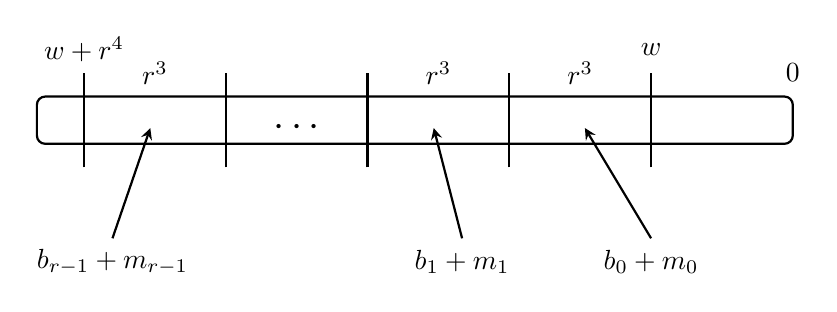
\begin{tikzpicture}[x=1.2cm, y=1cm, >=stealth]

    % Main horizontal rounded rectangle/bar
    \draw[thick, rounded corners=3pt] (1, 0) rectangle (9, 0.6);

    % Index labels
    \node at (1.5, 1.2) {$w+r^4$};
    \node at (9, 0.9) {$0$};
    \node at (7.5, 1.2) {$w$};

    % Vertical dividers cutting through the bar
    \draw[thick] (1.5, -0.3) -- (1.5, 0.9);
    \draw[thick] (3.0, -0.3) -- (3.0, 0.9);
    \draw[thick] (4.5, -0.3) -- (4.5, 0.9);
    \draw[thick] (6.0, -0.3) -- (6.0, 0.9);
    \draw[thick] (7.5, -0.3) -- (7.5, 0.9);

    % Segment labels (r^3) inside the divisions
    \node at (2.25, 0.9) {$r^3$};
    %\node at (3.75, 0.9) {$r^3$};
    \node at (5.25, 0.9) {$r^3$};
    \node at (6.75, 0.9) {$r^3$};

    % Pointed Arrows and Bottom Variables
    \draw[->, thick] (1.8, -1.2) -- (2.2, 0.2);
    \node at (1.8, -1.5) {$b_{r-1} + m_{r-1}$};

   % \draw[->, thick] (3.6, -1.2) -- (4.2, 0.2);
   % \node at (3.6, -1.5) {$b_r + m_r$};
    \node at (3.75, 0.2) {\Large $\cdots$};

    \draw[->, thick] (5.5, -1.2) -- (5.2, 0.2);
    \node at (5.5, -1.5) {$b_1 + m_1$};

    \draw[->, thick] (7.5, -1.2) -- (6.8, 0.2);
    \node at (7.5, -1.5) {$b_0 + m_0$};

\end{tikzpicture}
\caption{Resultado da multiplicação $x'\times m$. As somas $b_i+m_i$ estão
espaçadas em $r^3$ e vão de $w$ até $w+r^3$.\label{f:fusion-approx-sketch}}
\end{figure}

Feita essa multiplicação, teremos os bits importantes espalhados dessa forma, em
posições que conhecemos. Além disso, o resto dos bits podem conter qualquer
valor que não nos interessa. Por isso, aplicamos uma máscara com
\[
\sum_{i=0}^{r-1} 2^{b_i+m_i},
\]

preservando apenas os bits importantes. Por fim, um shift para a direita em
$b_0+m_0$ bits faz com que todos eles fiquem no intervalo de 0 a $O(r^4)$,
cabendo enfim em uma palavra de tamanho $w$.

Vale notar que, se quisermos na prática nos mantermos sempre dentro do tamanho de
palavra $w$, precisamos realizar esse shift antes mesmo da multiplicação.
Fazendo um shift de $b_0$ em $x'$ e de $m_0$ em $m$ nós garantimos que o
resultado da multiplicação já ficará dentro dos limites de uma palavra.   

\section{Concluindo a Fusion Tree}

Com o \textbf{Sketching Aproximado}, conseguimos obter uma bit-string de tamanho
$O(w^{4/5})$ contendo os bits importantes de uma chave $x$ em um padrão
previsível. Um nó possui $k=O(w^{1/5}$ chaves e, portanto, conseguimos reunir
seus sketchs aproximados em um array de tamanho $O(w)$. Isso permite realizar o
\textbf{Rank Paralelo} de uma consulta $q$ entre as chaves de um nó da Fusion
Tree.

Com a operação do \textbf{Rank Paralelo} garantida, a \textbf{Busca na Fusion
Tree} foi descrita na seção 6.3, e com ela obtemos em $O(1)$ por qual subárvore
vamos descer em cada nó da árvore. Relembrando, em uma Árvore B de ordem $b$ o
custo para atravessar a árvore é dado por $O(f(b)\log_b n$, onde $f(b)$ é o
trabalho feito em cada nó. No nosso caso, $f(b)=O(1)$ e a ordem é $b=w^{1/5}$.

Dessa forma, uma consulta de predecessor/sucessor na Fusion Tree leva tempo
$O(\log_w n)$.

\textit{[Fazer um exemplo completo com algumas chaves e uma busca]}
